\documentclass[main.tex]{subfiles}
\begin{document}


\chapter{Fazit}

Aus den erstellten Prototypen und der Evaluation sind viele Erkenntnisse zusammengekommen, die hier noch zusammengefasst werden. 

\section{Implementation}

\subsubsection{JasperReports}
Kleinere Probleme bei der Umsetzung haben die Entwicklung etwas behindert, wie die Probleme mit Bold. Der iReport zeigte das richtig an, aber es wurde nicht in die PDFs übernommen. Dennoch war iReport sehr gut: einfache Handhabung und gute Unterstützung für die Erstellung der Templates. Generierte Reports sind auch als kompilierte Jasper-Files noch verständlich.  


\subsubsection{Apache PdfBox}
Der Zeilenumbruch für einen langen Text muss selber entwickelt werden. Gleiches gilt für die Seitenumbrüche. Für lange Texte ist das eher umständlich. Es fehlt ein High-Level API, darum ist es eher schwierig, Templates zu erstellen, da diese immer auf der Basis von spezifischen Daten-Inputs basieren und eine dynamische Ansicht mit einem Flow-Pattern eher schwierig ist. Das Ausrichten von Textblöcken wird anhand der Seitengrösse programmiert, somit ist es auch im Textmodus schwierig, eine Tabelle mit mehrzeiligen Zelleninhalten zu kreieren.

Dennoch bietet sich Apache PDF an, um pixelgenaue Layouts zu erstellen, da die Texte mit Offset-Angaben ausgerichtet werden können.

\subsubsection{iText}
Es fühlt sich an, als schreibe man ein Worddokument. Die \acrlong{api} ist einfach und klar, Seiten werden automatisch neu generiert. Es benötigt keine Seitenangaben wie Rand und Grösse, da Standards diese bereits vorgeben. Ein Standard-Set an Fonts wird als Konstante mitgegeben. Der Hersteller bietet viele Beispiele und hilfreiche Blogs an. 
Die Positionierung einzelner Elemente kann über die Canvas-Funktionen ebenfalls erreicht werden, z.B. beim Definieren von Footer oder Header. 
iText lässt auch eine dokumentenübergreifende Fonteinstellung definieren, was die Entwicklung erleichtert. 
Doch auch hier ergeben sich Probleme mit den Fussnoten. Das Dokument müsste erneut bearbeitet werden, um die Anzahl Seiten zu kennen, da diese beim Erstellen noch nicht bekannt sind. Beim Erstellen einer neuen Seite ist die vorhergehende immer um eins kleiner, da beim Erstellen der Seite nicht bekannt war, dass eine weitere Seite dazukommt.

\section{Performance}



\subsection{Throughput}
% Welcher der Services hat am Meisten Durchsatz an den Tag gelegt ? 

Der höchste Durchsatz wurde mit ApachePDFBox erreicht, gefolgt von iText und dann Jasper-Reports. Die Analyse des Durchsatzes nach Bytes hat jedoch ergeben, dass dieser fast konstant blieb. Allenfalls ist dies ein Hinweis auf einen Engpass in der Netzwerkbandbreite.

\subsection{Latency}
Auch bei der Latency by Request ist Apache PDFBox am schnellsten. Die Verarbeitung kann bei den ersten zwei Szenarien unterhalb einer Sekunde durchgeführt werden, was bei JasperReports nicht der Fall ist. iText wiederum hat nur leicht längere Latenzzeiten.

\subsection{Verfügbarkeit}

Keiner der Tests ist jemals ausgefallen, es haben sich auch keine Fehler ereignet, die von JMeter als solche identifiziert wurden. Die meisten Tests haben sich über die Zeitspanne von 10 Stunden erstreckt, dabei haben die Logs ebenfalls keine Ausfälle nachgewiesen.

Dennoch hat JasperReports sehr lange Antwortzeiten, die ebenfalls zu Timeouts führen könnten, was somit die Verfügbarkeit einschränkt.


\section{Ressources}

\subsection{RAM}
Der Verbrauch von RSS-Memory ist sowohl bei iText als auch bei Apache PDFBox meist unterhalb der Memory-Quota. Der SWAP wird einzig von JasperReports genutzt und erklärt wohl die lange Verarbeitungszeit. Der SWAP wird nicht wieder freigegeben, was zu einer Memory-Blase führt.



\subsection{CPU}
Die CPU Last hat nur bei JasperReports durchgängige Spitzen angezeigt, Apache PDFBox hat hier wieder einmal ressourcenschonend gearbeitet. iText hat eine nicht erklärbare tiefe CPU Last im Szenario 3.


\section{Wer hat nun die beste Performance?}

\begin{figure}[!hb]
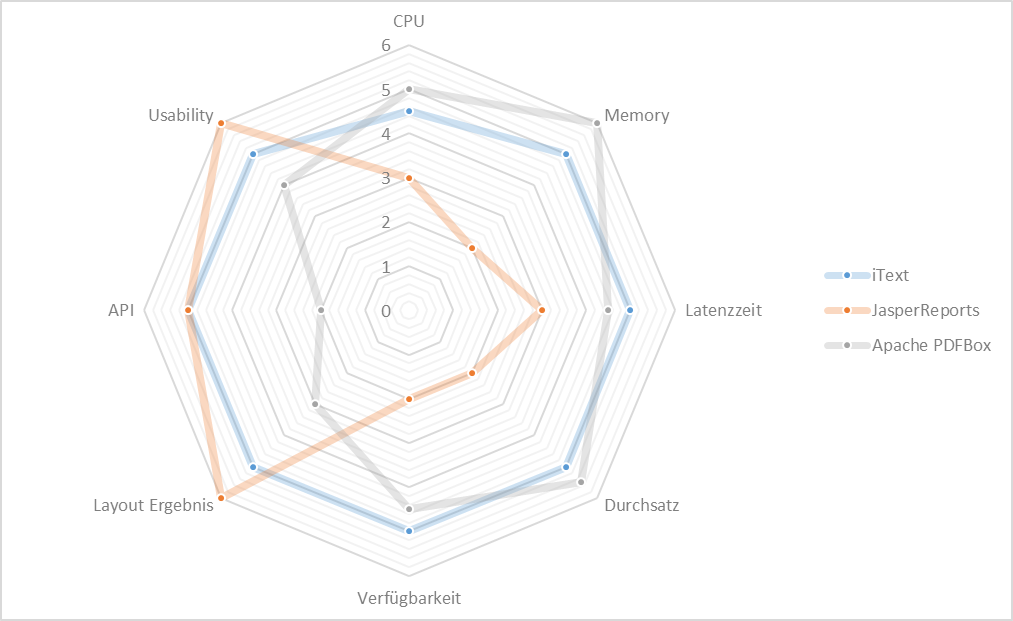
\includegraphics[width=\textwidth]{end/5_erfarhungsbericht/Netzdiagramm.png}
 \caption{Netzdiagramm nach Metrik}
 \label{figure:netzdiagrammMetriken}
\end{figure}

Würde man für diese Frage einzig und alleine die Daten des Durchsatzes nehmen, müsste man sagen, es sei im Durchschnitt Apache PDFBox. Trotz des Szenarios 3 erreicht dieser immer noch durchschnittlich 70 Anfragen pro Sekunde, gefolgt von iText mit 30 Anfragen pro Sekunde und dann JasperReports mit 14.5 Anfragen pro Sekunde.

Das 95\% Perzentil sagt wiederum, dass JasperReports der schnellste ist und das nur, weil das Szenario 3 die Antwortzeiten in die Höhe getrieben hat.

Pauschal lässt sich sagen, dass sich mit Apache PDFBox die höchste Performanz, Ressourcennutzung und Antwortzeiten erreichen lassen. Dennoch haben auch die anderen \acrshort{osre}s gute Seiten, die in verschiedenen Anwendungsfällen besser einzusetzen sind. In der Abbildung \ref{figure:netzdiagrammMetriken} lassen sich die Tendenzen der jeweiligen \acrshort{osre} erkennen.

\subsection{Apache PDFBox}

Diese hat klare Stärken, was die technische Performance angeht. 
Die Umsetzung ist klar auch historisch geprägt. Es ist ein Tool primär zur Extraktion von Daten und nicht für die Erstellung von Reports gedacht, was es auch so performant macht. Das geeignete Einsatzgebiet im Umfeld von Reporterstellung liegt auf dem Gebiet von statischen Layouts wie Flugtickets oder Konzertkarten.


\subsection{iText}

iText wurde genau dafür kreiert, um Reports zu generieren. Dies ist klar erkennbar an dem versatillen und umfangreichen \acrshort{api}. Es beherrscht auch den komplexeren PDF-Aufbau ohne Performanceverlust. Für einen Online-Einsatz wird es als brauchbar empfunden. Das API ist gut genug, um Reports leicht verständlich zu codieren, und bleibt darum wartbar.

\subsection{JasperReports}
Es gibt klare Vorteile bei visuell aufbereiteten Reports, leider hat aber dieser Vorteil keine nutzbare Performance für eine Online-Verarbeitung gezeigt. Dies bedeutet: JasperReports ist für einen Einsatz in einem Microservice nur sehr bedingt geeignet. Ein geeignetes Einsatzgebiet wären zeitlich klar definierte Reportgenerierungen. Oder auch wenn komplexe Reports womöglich von Nicht-Entwicklern definiert werden sollen, ist iReport dafür ein geeignetes Hilfsmittel.

\section{Ausblick}

Aus den Peformance-Messungen entstanden einige Fragen im Zusammenhang mit der Implementation, die noch zu adressieren ist, wie z.B.: 
\begin{itemize}  
    \item Sind Engpässe in Applikation oder Netzwerk Ursachen für die schlechte Performance? 
    \item Sind Fehler in der Applikation, die einen unnötigen Programmcode ausführen?
    \item Sind Einstellungen möglich, um Zugriffe auf Dateien wie Bilder zu verbessern?
\end{itemize}
Und in dieser Arbeit nicht addressierbare Fragen bezüglich Skalierbarkeit der PaaS.
\begin{itemize}  
    \item Mit welcher Anzahl Server können X Anzahl User performant bedient werden?
    \item Wie verhält sich das Auto-Scaling?
    \item Wie gut funktioniert das Load Balancing ? 
\end{itemize}
Diese Fragen könnten in einer weiteren Arbeit vertieft werden. 

\end{document}